\chapter{Base teórica}
\label{cap:base-teorica}

La reconstrucción de cuerpos u objetos en 3D a partir de un sensor RGBD se consigue gracias al uso de métodos de registro que realizan cálculos de correspondencias entre dos vistas distintas.
Es decir, dado un conjunto de datos de entrada, donde cada entrada son capturas de nubes de puntos de un mismo cuerpo realizadas desde distintos ángulos, el método de registro se encargará de encontrar una transformación que alinee estas nubes de puntos para finalmente reconstruir el cuerpo entero.
Esta transformación no es más que una combinación de rotaciones y traslaciones en los ejes de coordenadas $\mathbf{X}$, $\mathbf{Y}$, $\mathbf{Z}$ sobre la nube de puntos.

\section{Métodos de registro}
\label{sec:metodos-de-registro}

Los métodos de registro tratan de encontrar una correspondencia entre la posición de los puntos de una nube de puntos y otra, emparejándolos para calcular de esta forma la transformación global que corresponda de mejor manera entre los dos conjuntos de nube de puntos.
Estos métodos realizan cálculos en ocasiones de forma iterativa, para encontrar la mejor correspondencia entre los puntos y así estimar la transformación que consiga alinear ambas vistas.

\begin{figure}[h]
    \centering
    \begin{subfigure}[t]{0.33\textheight}
    	\centering
        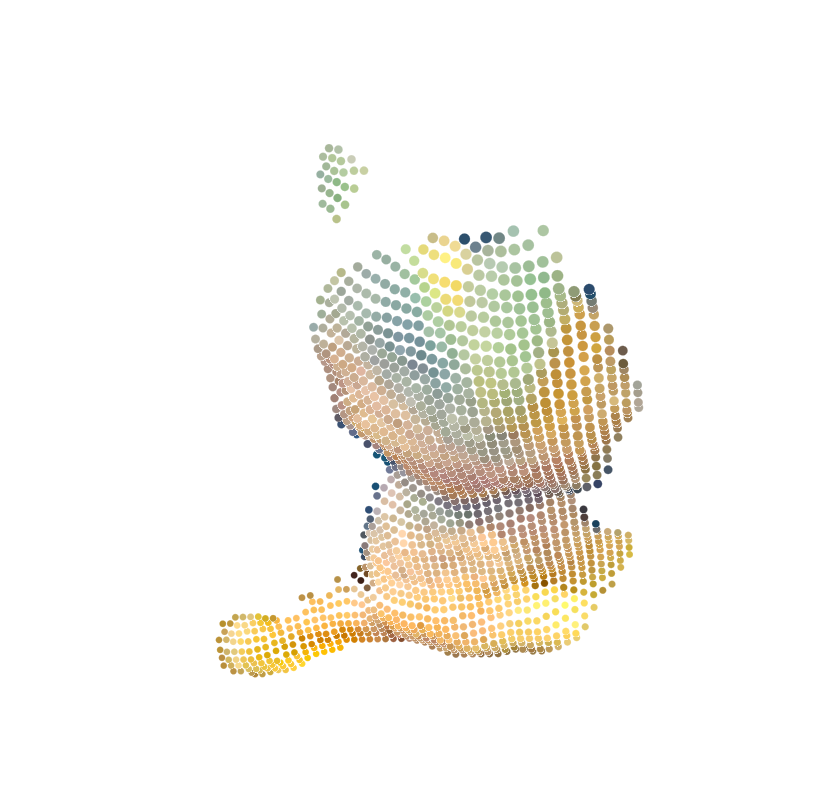
\includegraphics[height=4cm]{archivos/metodo-registro-explicacion-modelo-2.png}
        \caption{Captura del modelo.}
        \label{fig:metodo-registro-explicacion-modelo}
    \end{subfigure}
    \begin{subfigure}[t]{0.33\textheight}
    	\centering
        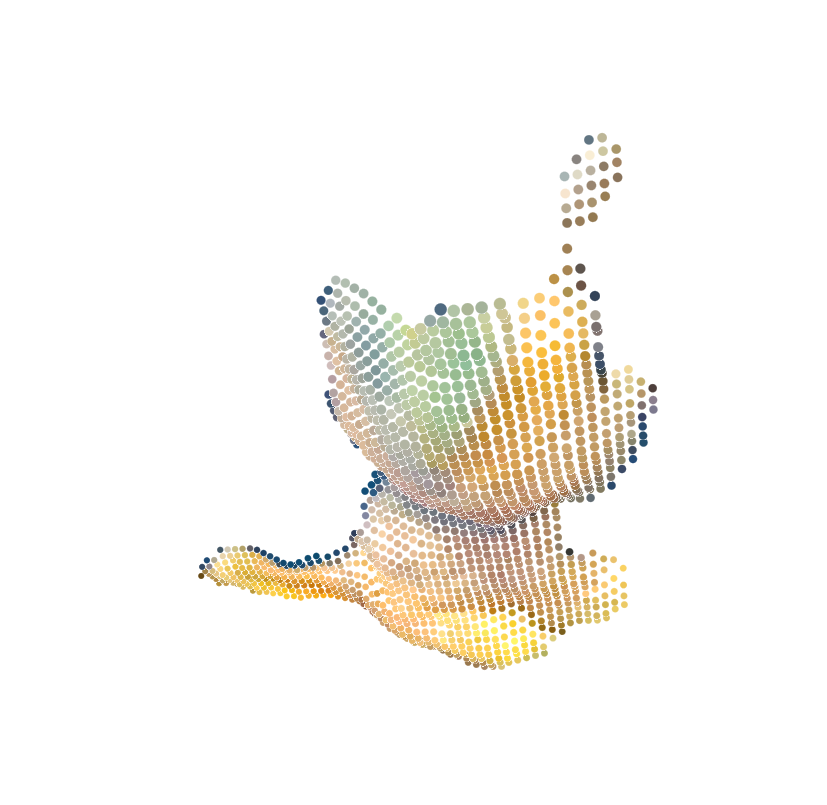
\includegraphics[height=4cm]{archivos/metodo-registro-explicacion-escena-2.png}
        \caption{Captura de la escena.}
        \label{fig:metodo-registro-explicacion-escena}
    \end{subfigure}
    \begin{subfigure}[t]{0.33\textheight}
    	\centering
        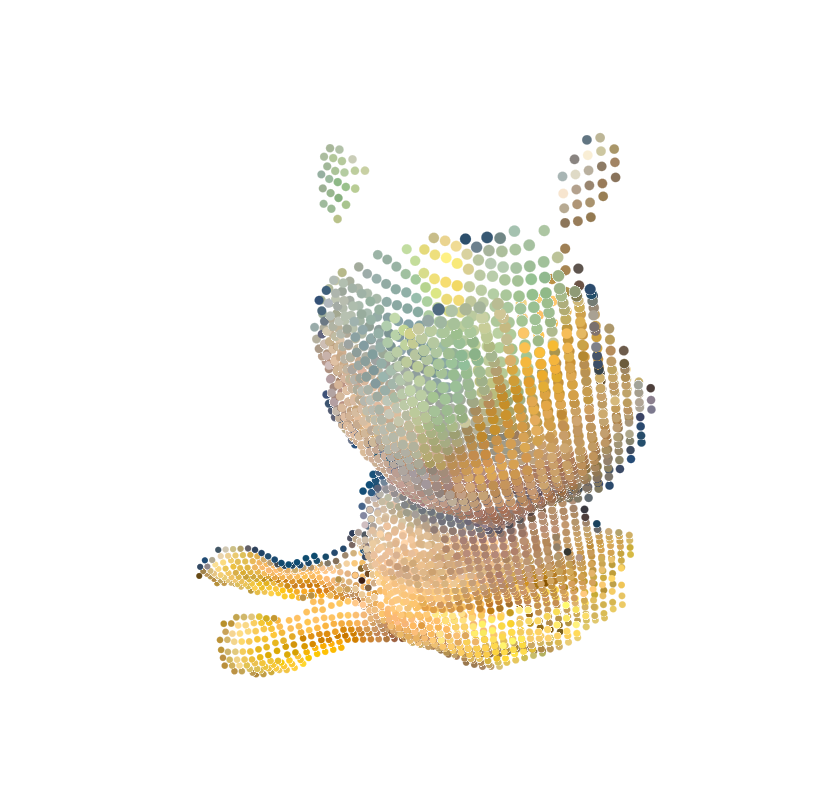
\includegraphics[height=4cm]{archivos/metodo-registro-explicacion-superpuesto-2.png}
        \caption{Modelo y escena superpuestos.}
        \label{fig:metodo-registro-explicacion-superpuesto}
    \end{subfigure}
    \begin{subfigure}[t]{0.33\textheight}
    	\centering
        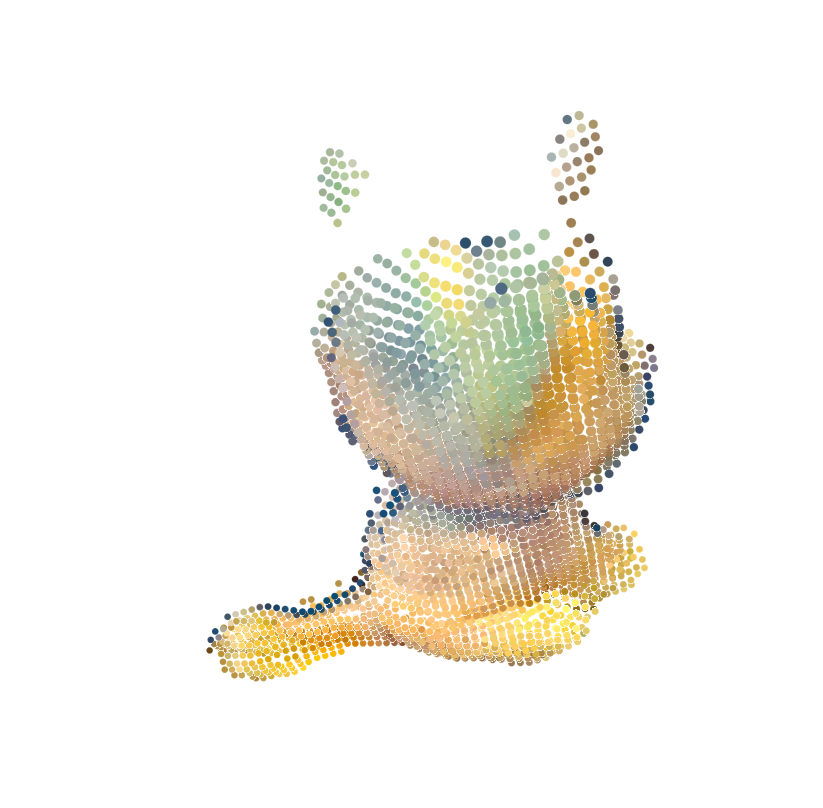
\includegraphics[height=4cm]{archivos/metodo-registro-explicacion-alineacion-2.png}
        \caption{Escena alineada con el modelo.}
        \label{fig:metodo-registro-explicacion-alineacion}
    \end{subfigure}
    \caption{Ejemplo de alineación de una escena con un modelo.}
    \label{fig:metodo-registro-explicacion}
\end{figure}

Como podemos ver en la Figura \ref{fig:metodo-registro-explicacion}, dado dos entradas de nubes de punto, el modelo y la escena, obtenemos su alineación a través de un método de registro.
Normalmente a la nube de puntos de referencia con la que se tratará de alinear el resto de nubes de puntos recibe el nombre de modelo.
Las nubes de puntos que se tratan de emparejar reciben el nombre de escena.
Cuando aplicamos un método de registro sobre una escena (Figura \ref{fig:metodo-registro-explicacion-escena}) y tomamos como referencia un modelo (Figura \ref{fig:metodo-registro-explicacion-modelo}) lo que conseguiremos es transformar la escena para que quede alineada y así forme parte del modelo (Figura \ref{fig:metodo-registro-explicacion-alineacion}).
De esta forma, gracias a la alineación de la escena sobre el modelo, conseguimos que el modelo quede más completo.

\begin{figure}[h]
    \centering
    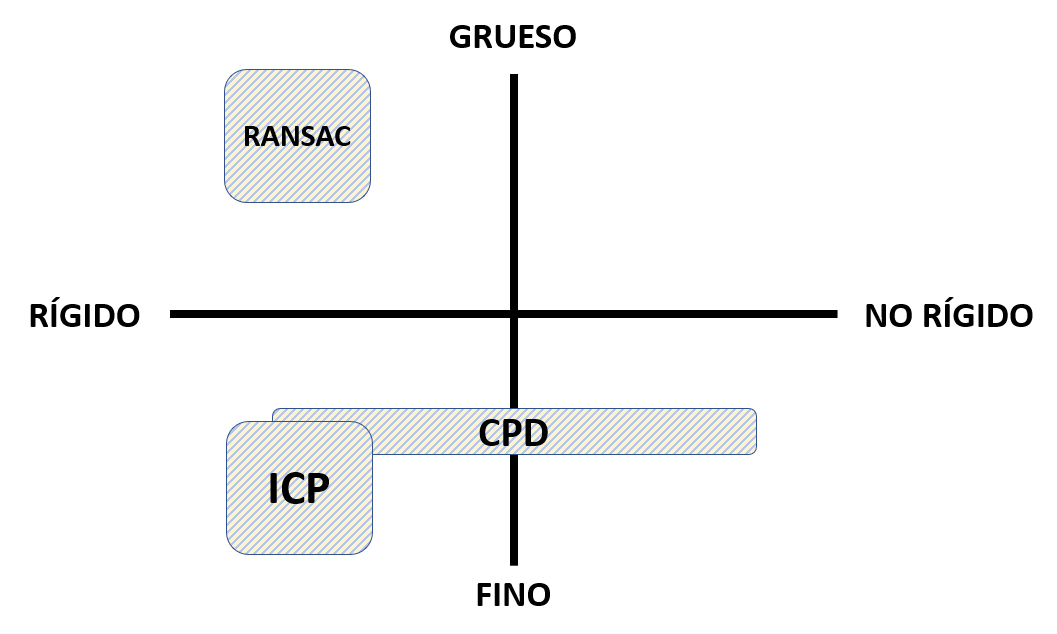
\includegraphics[height=6cm]{archivos/diagrama-tipos-registro.png}
    \caption{Diagrama tipos de registro.}
    \label{fig:diagrama-tipos-registro}
\end{figure}

En la Figura \ref{fig:diagrama-tipos-registro} podemos ver un diagrama que sitúa algunos de los métodos de registros de los que hablaremos en este \gls{tfg} en función de sus características.
Podemos ver que un método de registro se puede diferenciar por ser de grano grueso o grano fino, y por el tipo de registro que se está utilizando para alinear los datos: rígido o no rígido.
    
Los métodos de grano grueso suelen utilizarse como paso inicial en el registro debido a que suelen ser poco precisos, pero ofrecen una buena aproximación inicial para vistas muy separadas entre sí.
Estos métodos suelen muestrear los datos y utilizan métodos basados en detección y descripción de características para intentar reducir la cantidad de puntos tanto de la escena como del modelo.
Una característica (keypoint) tiene una posición y un descriptor que describe
ese keypoint.
Las características proceden de la captura en sí ya sea una imagen \gls{2d} o una nube de puntos (imagen \gls{3d}).
En este paso de detección de características se intenta detectar las partes distintivas de un objeto en los conjuntos de datos, como formas, regiones cerradas, contornos, líneas, etc.
Una vez detectadas las partes del objeto se representa como un conjunto de valores normalmente llamados descriptores de
características.
Tras la detección y descripción de características, se buscan correspondencias entre las mismas y finalmente una estimación de la transformación.

El método basado en características más utilizado para encontrar la transformación entre correspondencias está basado en el paradigma \gls{ransac}, publicado por primera vez por \cite{Fischler1981}.
\gls{ransac} es un método iterativo para calcular los parámetros de un modelo matemático de un conjunto de datos observados que contiene valores atípicos.
Es un algoritmo no determinista en el sentido de que produce un resultado razonable solo con una cierta probabilidad, mayor a medida que se permiten más iteraciones.
En cada iteración del algoritmo, se selecciona aleatoriamente un subconjunto de correspondencias a los que se les aplica una matriz de transformación.
Los datos restantes se testean con el modelo aplicado de manera que si su error está por encima de un umbral se eliminan de los datos seleccionados, de esta forma se descartan los puntos con errores extremadamente altos (outliers).
En la Figura \ref{fig:ransac-ejemplo} podemos ver un ejemplo de alineación con imágenes \gls{2d} utilizando \gls{ransac}.
En la subfigura \ref{fig:ransac-ejemplo-alineado-bien} podemos ver un ejemplo de resultado de una iteración que ha tenido buena probabilidad con la correspondencia entre el subconjunto de puntos seleccionados (subfigura \ref{fig:ransac-ejemplo-correspondencias}).
En la subfigura \ref{fig:ransac-ejemplo-alineado-mal} podemos ver un ejemplo de una iteración que ha partido de una mala correspondencia entre los subconjuntos de los puntos seleccionados.
Este proceso se repite varias veces, finalmente se utilizará la iteración que mejor solución presente como aproximación inicial para un método de registro de grano fino.

\begin{figure}[h!]
    \centering
    \begin{subfigure}[t]{0.5\textheight}
        \centering
        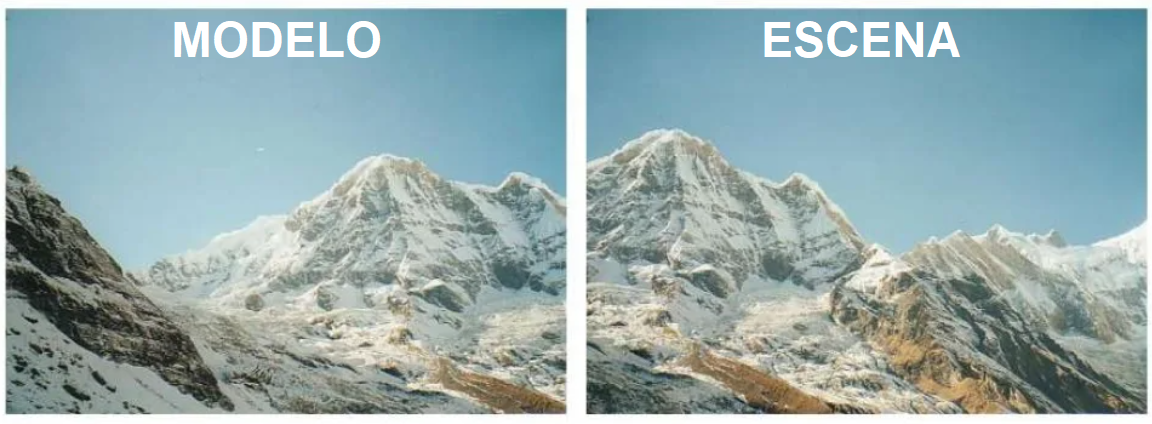
\includegraphics[height=3cm]{archivos/ransac-ejemplo.png}
        \caption{Dos capturas en 2D.}
        \label{fig:ransac-ejemplo-capturas}
    \end{subfigure}
    \begin{subfigure}[t]{0.5\textheight}
        \centering
        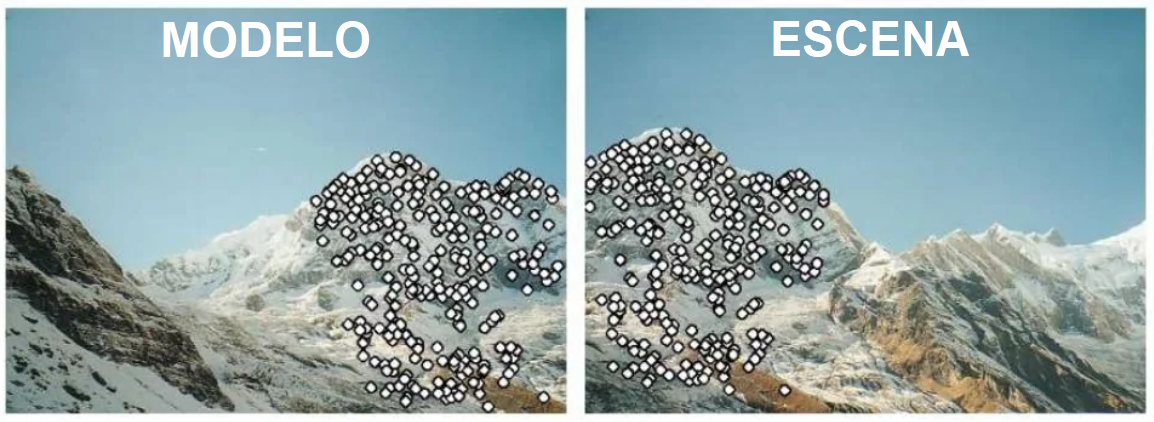
\includegraphics[height=3cm]{archivos/ransac-ejemplo-caracteristicas.png}
        \caption{Búsqueda de características en las capturas.}
        \label{fig:ransac-ejemplo-caracteristicas}
    \end{subfigure}
    \begin{subfigure}[t]{0.5\textheight}
        \centering
        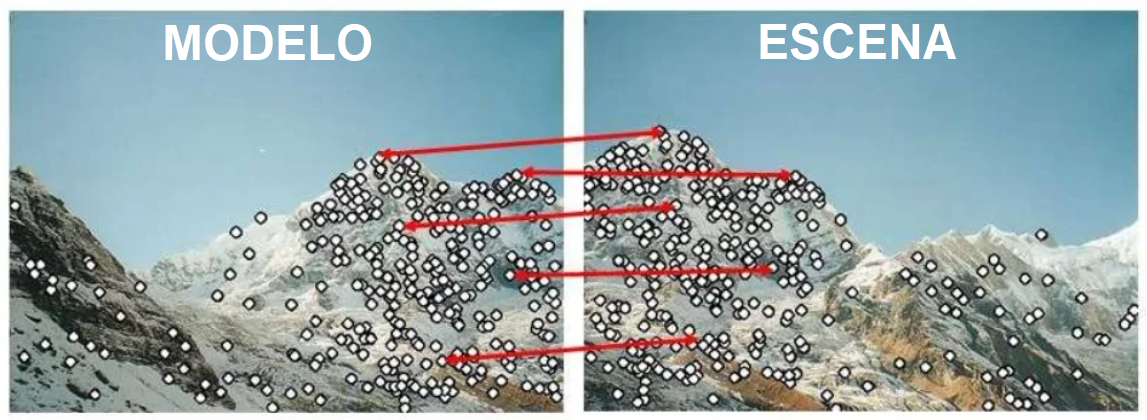
\includegraphics[height=3cm]{archivos/ransac-ejemplo-correspondencias.png}
        \caption{Búsqueda de correspondencias en las capturas.}
        \label{fig:ransac-ejemplo-correspondencias}
    \end{subfigure}
    \begin{subfigure}[t]{0.33\textheight}
        \centering
        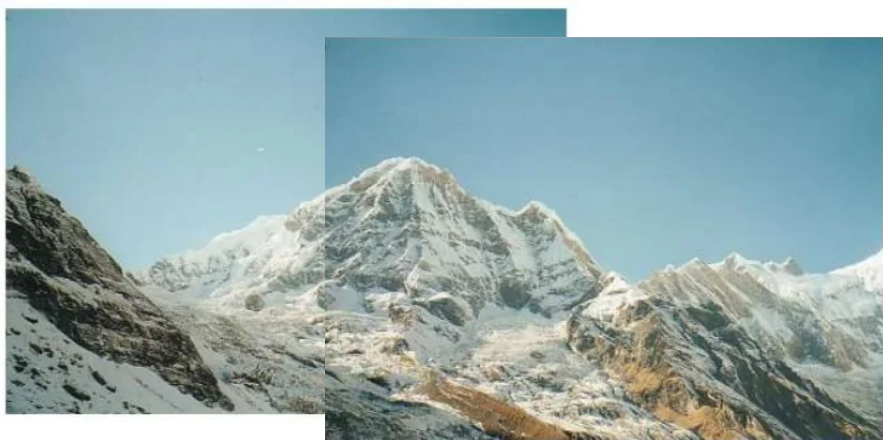
\includegraphics[height=3.5cm]{archivos/ransac-ejemplo-alineado-bien.png}
        \caption{Ejemplo de alineación con correspondencias muy buenas.}
        \label{fig:ransac-ejemplo-alineado-bien}
    \end{subfigure}
    \begin{subfigure}[t]{0.33\textheight}
        \centering
        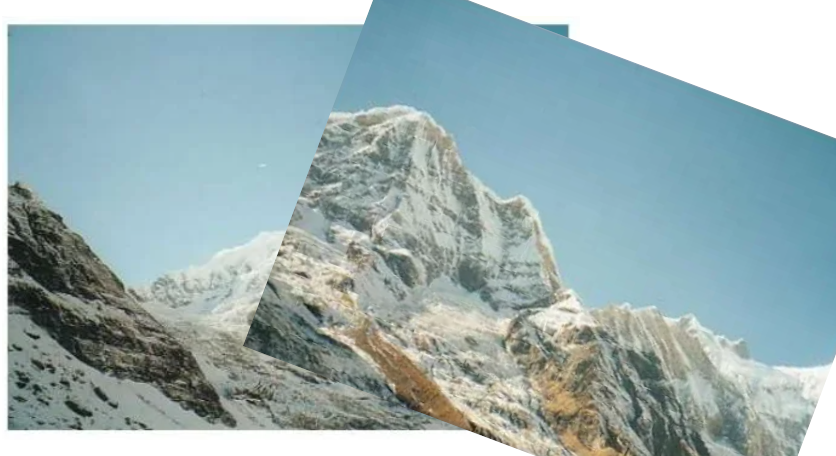
\includegraphics[height=3.5cm]{archivos/ransac-ejemplo-alineado-mal.png}
        \caption{Ejemplo de alineación con correspondencias muy malas.}
        \label{fig:ransac-ejemplo-alineado-mal}
    \end{subfigure}
    \caption{Ejemplo de alineación de una escena usando RANSAC.}
    \label{fig:ransac-ejemplo}
\end{figure}

Los métodos de grano fino se usan normalmente cuando se necesitan resultados más precisos.
Por lo general, estos métodos necesitan el resultado de un registro de grano grueso previo como dato inicial del que partir.
Cuando se le aplica el resultado de un método de grano grueso a la escena, esta se encontrará más próxima al modelo, facilitando así la ejecución de un método de grano fino.
Sin embargo, no siempre es necesario una alineación previa si las nubes de puntos que se intentan alinear ya están lo suficientemente cerca.
Por ejemplo, cuando se usa una frecuencia de capturación en el sensor muy alta, y el movimiento entre dos capturas consecutivas es muy pequeño. 

Como conclusión entre los métodos de grano grueso y fino, los métodos de registro fino se suele utilizar para refinar un registro en el
que la escena y el modelo se encuentran muy próximos, en contraste con los métodos de grano grueso que se suelen utilizar para distancias mayores con la finalidad de aproximar la escena al modelo sin ser del todo preciso.

Por otra parte, los métodos de registro también se pueden diferenciar entre métodos de registro rígidos y métodos de registro no rígidos.
Cuando hablamos de un objeto o cuerpo no rígido, nos referimos a un objeto o cuerpo articulado o deformable.
El registro rígido se utiliza cuando la diferencia entre modelo y escena consiste en una matriz de transformación, es decir, la escena sobre el objeto se ha rotado o movido respecto al modelo sobre el objeto, pero en ambos casos el objeto es el mismo y mantiene la misma forma.
Cuando hablamos de un registro no rígido es porque el objeto de la escena puede haber sido deformado, además de rotado o movido respecto al modelo.

\subsection{Métodos de registro rígidos, ICP}

El método de registro rígido más utilizado es el \gls{icp} \cite{Besl1992}. Es un método de propósito general, independiente de la representación y cuyo cometido es encontrar la transformación entre una nube de puntos y otra, minimizando los errores entre los puntos emparejados de ambas nubes.
Este método trata de realizar el registro de nubes de puntos de manera eficiente desde el punto de vista computacional.
Si las nubes de puntos se encuentran lo suficientemente cerca, el algoritmo es capaz de proporcionar  muy buenos resultados en la mayoría de casos.

\begin{figure}[h]
    \centering
    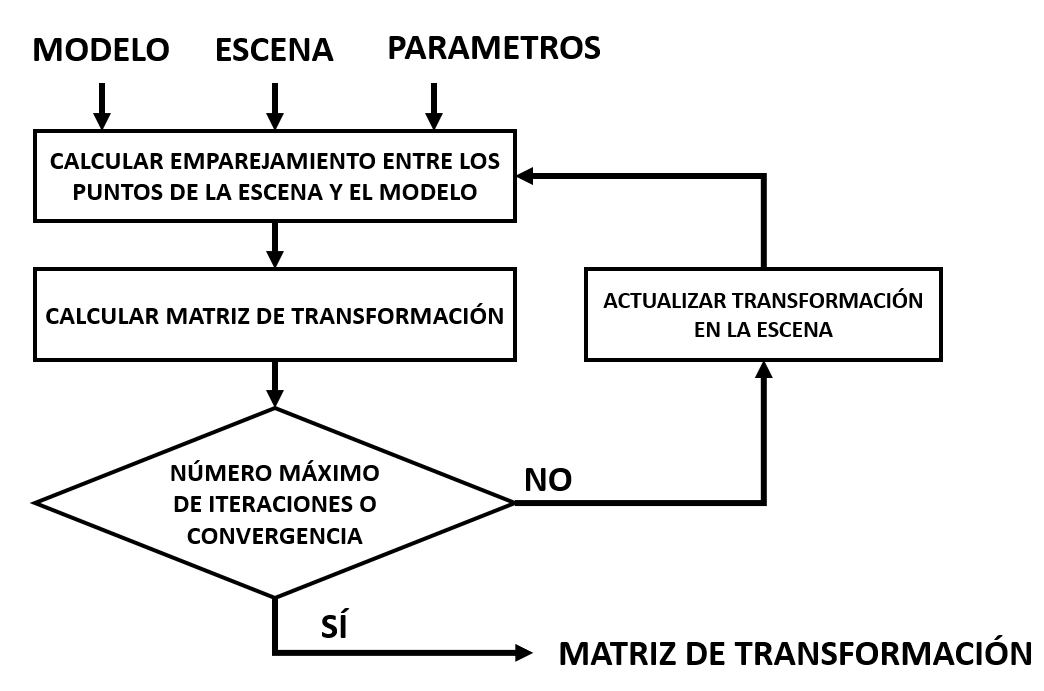
\includegraphics[height=8cm]{archivos/esquema-algoritmo-icp.png}
    \caption{Diagrama del algoritmo ICP.}
    \label{fig:esquema-algoritmo-icp}
\end{figure}

En la Figura \ref{fig:esquema-algoritmo-icp} podemos ver un esquema del funcionamiento del algoritmo \gls{icp}.
Este algoritmo recibe como parámetros de entrada la nube de puntos de la escena (fuente) y la nube de puntos del modelo (destino), además de los parámetros de configuración del algoritmo.
El algoritmo parte de la escena, que es la nube de puntos a alinear, y aplica diversas transformaciones con el objetivo de acercarse a la nube destino, el modelo.
El proceso se realiza de forma iterativa, partiendo en cada nueva iteración de la transformación anterior, hasta que finalmente la nube de puntos converge con el destino.
El resultado de aplicar el algoritmo \gls{icp} es la nube de puntos de la escena alineada, a la vez que una matriz de transformación final.
Si esta matriz de transformación la aplicamos sobre la nube de puntos de la escena original, obtendremos una nube de puntos de escena alineada con la nube de puntos del modelo.

Además, al método \gls{icp} original se pueden aplicar diferentes variaciones con la finalidad de mejorar su robustez.
Por ejemplo, se le puede añadir un parámetro para indicar el límite máximo de distancia para la correspondencia entre puntos, es decir, un valor que indique el radio de distancia desde cada punto en la nube de puntos de origen (escena) en el que la búsqueda de vecinos intentará encontrar un punto correspondiente en la nube de puntos de destino (modelo).
Este parámetro puede ser muy importante ya que limitar esta distancia ayuda en el rendimiento (cuanto menor sea el radio más rápido será) y puede evitar que el resultado no converja si la diferencia entre ambas nubes de puntos es muy grande.

\begin{figure}[h]
    \centering
    \begin{subfigure}[t]{0.33\textheight}
    	\centering
        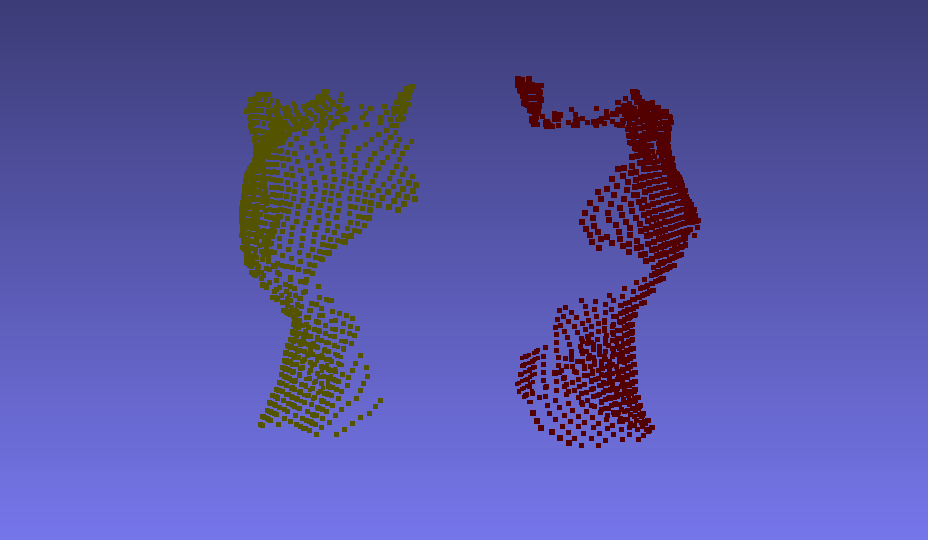
\includegraphics[height=4cm]{archivos/metodo-registro-explicacion-superpuesto-2-puntos.png}
        \caption{Modelo y escena superpuestos sin alinear.}
    \end{subfigure}
    \begin{subfigure}[t]{0.33\textheight}
    	\centering
        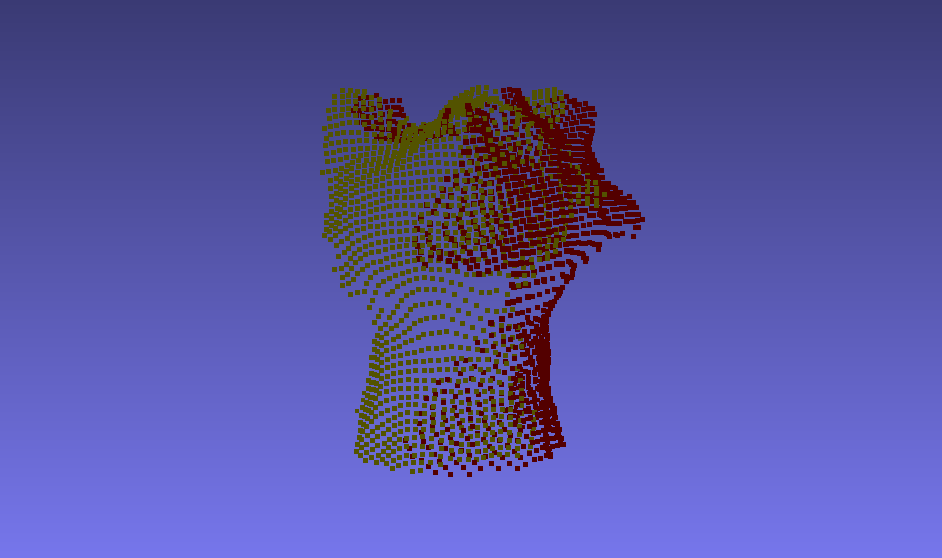
\includegraphics[height=4cm]{archivos/metodo-registro-explicacion-alineacion-puntos.png}
        \caption{Modelo y escena superpuestos alineados.}
    \end{subfigure}
    \caption{Ejemplo de captura de escena muy alejada al modelo.}
    \label{fig:modelo-escena-alejados-ejemplo}
\end{figure}

En la Figura \ref{fig:modelo-escena-alejados-ejemplo} podemos ver un caso donde gran parte de la nube de puntos de la escena no corresponden con el modelo, por tanto son pocos la cantidad de puntos que deberían coincidir entre ambas nubes.
En este caso, aplicar un umbral de distancia máxima entre correspondencias será muy útil para que el algoritmo \gls{icp} descarte los emparejamientos entre los puntos más lejanos.
También son importantes parámetros como el número de iteraciones máximas o el valor umbral para el error medio de emparejamiento que definirá la cantidad de iteraciones que el algoritmo \gls{icp} debe realizar para obtener la convergencia entre escena y modelo.

\subsection{Métodos de registro no rígidos, CPD}
\label{subsec:metodos-registro-no-rigido-cpd}

Mientras que una transformación rígida solo permite la traslación, rotación y escalado de la escena, la transformación no rígida permite tanto transformar afines, articulares y sesgos anisotrópicos.
Las aproximaciones simplistas de transformación no rígida verdadera, incluidos los modelos polinómicos y afines por partes, a menudo son inadecuadas para la alineación correcta y pueden producir correspondencias erróneas.
También suelen tener una alta complejidad computacional.
Además, debido al gran número de parámetros de transformación, los métodos de registro de nubes de puntos no rígidas tienden a ser sensibles al ruido y a los valores atípicos y es probable que converjan en mínimos locales.
Las degradaciones como el ruido, los valores atípicos y los puntos faltantes complican significativamente el problema.
Los valores atípicos son los puntos que se extraen incorrectamente de la imagen, estos valores atípicos no tienen correspondencias en el otro conjunto de puntos.

\gls{cpd} es un método de registro desarrollado originalmente por \cite{Myronenko2010}.
\gls{cpd} presenta un robusto algoritmo de registro de nubes de puntos probabilístico para transformaciones rígidas y no rígidas.
Mientras que \gls{icp} minimiza las distancias punto a punto, \gls{cpd} utiliza un \gls{mmg} para minimizar el error entre un punto y todos los demás puntos.
La alineación de dos nubes de puntos se considera como un problema de estimación de densidad de probabilidad, donde una nube de puntos representa los centroides del \gls{mmg} y el otro representa los puntos de datos.
Los centroides de \gls{mmg} se ajustan a los datos maximizando la probabilidad.
En el punto óptimo, las nubes de puntos se alinean y la correspondencia se obtiene usando las probabilidades posteriores de los componentes \gls{mmg}.
El núcleo del algoritmo es obligar a los centroides \gls{mmg} a moverse coherentemente como un grupo, lo que preserva la estructura topológica de los conjuntos de puntos.

El hecho de utilizar el \glsentrylong{mmg} entre punto y punto conlleva un rendimiento muy intensivo desde el punto de vista computacional.
Este algoritmo utiliza \gls{fgt}, una librería para acelerar las transformaciones gaussianas, también desarrollado por \cite{Myronenko2010}.
No obstante, tanto el algoritmo \gls{cpd} como los cálculos de errores subyacentes tardan mucho tiempo, a pesar de utilizar \gls{fgt}.

\section{Matriz de transformación 3D}

Como este \gls{tfg} utiliza tipos de datos \gls{3d}, los conceptos que se exponen serán enfocados a este tipo de datos.
La matriz de transformación \citep{wiki:transformation-matrix} es el resultado que obtenemos tras aplicar el método de registro.
Con la matriz de transformación, podemos transformar la nube de puntos de la escena y alinearla con la nube de puntos modelo.
La matriz de transformación se aplica directamente sobre una nube de puntos para transformarla.
Una nube de puntos es una matriz de $3\times\mathbf{N}$ donde $\mathbf{N}$ es la cantidad de puntos, para cada uno de los cuales tenemos el valor $\mathbf{X}$, $\mathbf{Y}$, $\mathbf{Z}$.\footnote{Una nube de puntos RGB, es decir, con color, será de $6\times\mathbf{N}$: los valores de posición $\mathbf{X}$, $\mathbf{Y}$, $\mathbf{Z}$; y los valores de color $\mathbf{R}$, $\mathbf{G}$, $\mathbf{B}$.
En estos casos, las matrices de transformación sólo se aplicarán a los valores $\mathbf{X}$, $\mathbf{Y}$, $\mathbf{Z}$.}
Al aplicar la matriz sobre la nube de puntos conseguimos transformarla, rotando y trasladando los puntos en su interior, con la finalidad, en este caso, de alinearlos con otra nube de puntos.

Una matriz de transformación está compuesta de una matriz de rotación y una matriz de traslación.

La matriz de rotación \citep{wiki:rotation-matrix} es una matriz $3\times3$ que contiene el valor por el que se necesita multiplicar cada uno de los puntos de una nube de puntos para ser rotada.
Una rotación básica consiste en una rotación que afecte solamente a uno de los ejes de coordenadas.
En la Ecuación \ref{eq:matrices-rotacion-basicas} podemos ver las tres matrices de rotación básicas para cada uno de los ejes, donde $\theta$ indica el ángulo con el que los ejes van a rotar.
Por ejemplo, si queremos rotar nuestra nube de puntos 15º grados en el eje $\mathbf{X}$, habría que aplicar la matriz de rotación $\mathbf{R}_{x}(15)$ a nuestra nube de puntos.
Tras multiplicar nuestra nube de puntos $3\times\mathbf{N}$ por esta matriz, obtendremos una nueva nube de puntos con nuevos valores que resultará en la misma nube de puntos rotada 15º en el eje $\mathbf{X}$, como se puede ver en el ejemplo de la Figura \ref{fig:modelo-rotado-15-eje-x}.

\begin{customequation}[h!]
    \begin{equation}
        \begin{aligned}
            \mathbf{R}_{x}(\theta)
            =
            \begin{vmatrix}
                1 & 0 & 0 \\
                0 & \cos\theta  & -\sin\theta \\
                0 & \sin\theta & \cos\theta
            \end{vmatrix}
            \\
            \\
            \mathbf{R}_{y}(\theta)
            =
            \begin{vmatrix}
                \cos\theta & 0 & \sin\theta \\
                0 & 1  & 0 \\
                -\sin\theta & 0 & \cos\theta
            \end{vmatrix}
            \\
            \\
            \mathbf{R}_{z}(\theta)
            =
            \begin{vmatrix}
                \cos\theta  & -\sin\theta & 0 \\
                \sin\theta & \cos\theta  & 0 \\
                0 & 0 & 1
            \end{vmatrix}
        \end{aligned}
    \end{equation}
    \caption{Matrices de rotación básicas.}
    \label{eq:matrices-rotacion-basicas}
\end{customequation}

\begin{figure}[h]
    \centering
    \begin{subfigure}[t]{0.33\textheight}
    	\centering
        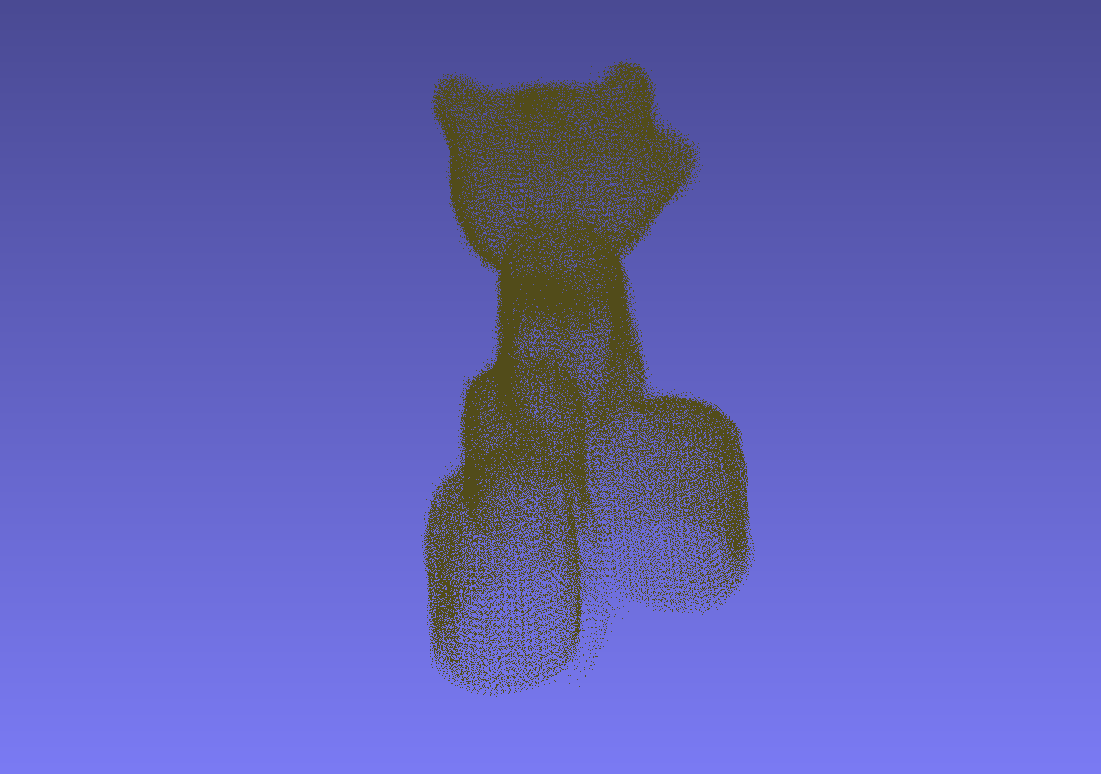
\includegraphics[height=4cm]{archivos/rotacion-15-original.png}
        \caption{Modelo 3D original.}
    \end{subfigure}
    \begin{subfigure}[t]{0.33\textheight}
    	\centering
        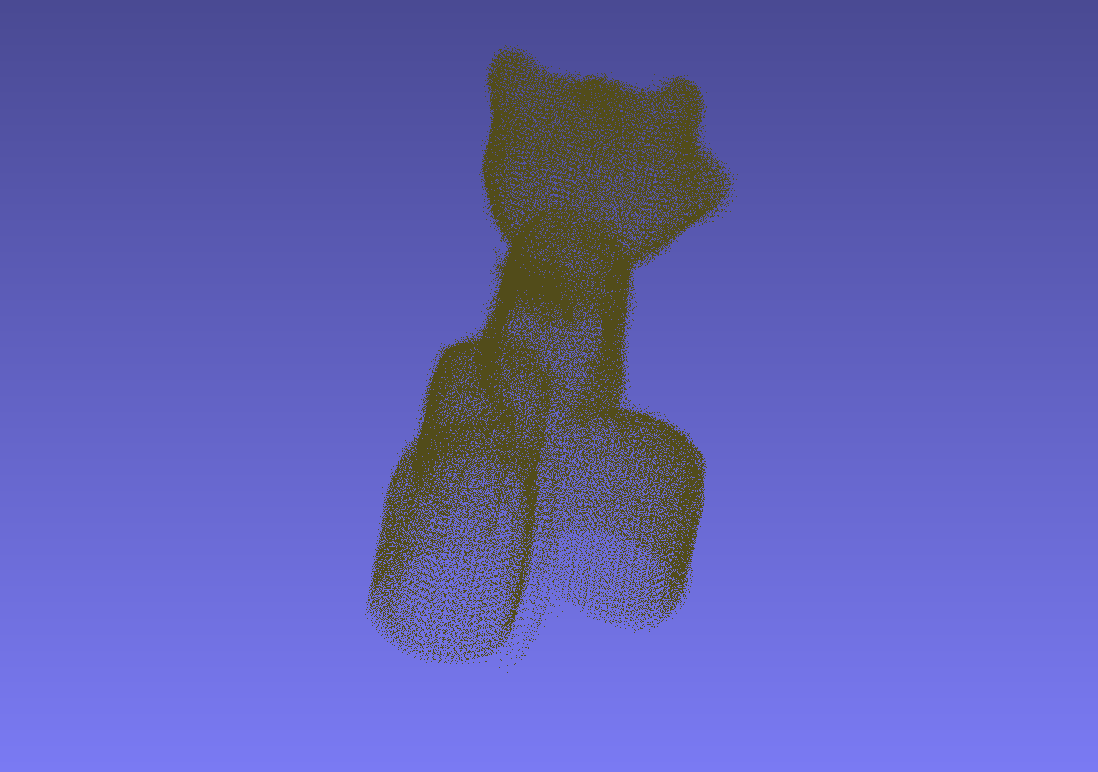
\includegraphics[height=4cm]{archivos/rotacion-15-rotado.png}
        \caption{Modelo 3D rotado 15º en el eje $\mathbf{X}$.}
    \end{subfigure}
    \caption{Rotación de 15º de un modelo 3D en el eje $\mathbf{X}$.}
    \label{fig:modelo-rotado-15-eje-x}
\end{figure}

La traslación \citep{wiki:translation-matrix} es una transformación geométrica que permite mover cada punto de la nube de puntos la misma distancia y en la misma dirección. Este movimiento puede ser representado en forma de vector o de matriz (Ecuación \ref{eq:vector-matriz-traslacion}).

\begin{customequation}[h!]
    \begin{equation}
        \mathbf{T}_{v}
        =
        \begin{vmatrix}
            v_{x} \\
            v_{y} \\
            v_{z}
        \end{vmatrix}
        \hspace{0.5cm}
        \mathbf{T}_{v}
        =
        \begin{vmatrix}
            1 & 0 & 0 & v_{x} \\
            0 & 1 & 0 & v_{y} \\
            0 & 0 & 1 & v_{z} \\
            0 & 0 & 0 & 1 \\
        \end{vmatrix}
    \end{equation}
    \caption{Vector y matriz de Traslación.}
    \label{eq:vector-matriz-traslacion}
\end{customequation}

La traslación es una transformación afín sin puntos fijos, sin embargo, la multiplicación en las matrices siempre tienen su origen como punto fijo.
Para solucionar este inconveniente, al vector de 3 dimensiones $\mathbf {v}=(v_{x},v_{y},v_{z})$ se le añade una dimensión más $\mathbf {v}=(v_{x},v_{y},v_{z},1)$, de esta forma conseguimos trabajar utilizando coordenadas homogéneas para representar la traslación en un espacio vectorial con multiplicación de matrices.
Como podemos ver en la Ecuación \ref{eq:matriz-traslacion-aplicada}, se está multiplicando una matriz de traslación por uno de los puntos de una nube de puntos.
El resultado de esta multiplicación consiste en ese mismo punto sumándole el movimiento de la matriz de traslación.

\begin{customequation}[h!]
    \begin{equation}
        \mathbf{T}_{v}
        \mathbf{p}
        =
        \begin{vmatrix}
            1 & 0 & 0 & v_{x} \\
            0 & 1 & 0 & v_{y} \\
            0 & 0 & 1 & v_{z} \\
            0 & 0 & 0 & 1 \\
        \end{vmatrix}
        \begin{vmatrix}
            p_{x} \\
            p_{y} \\
            p_{z} \\
            1 \\
        \end{vmatrix}
        =
        \begin{vmatrix}
            p_{x} + v_{x} \\
            p_{y} + v_{y} \\
            p_{z} + v_{z} \\
            1 \\
        \end{vmatrix}
        = p + v
    \end{equation}
    \caption{Matriz de Traslación aplicada a un punto.}
    \label{eq:matriz-traslacion-aplicada}
\end{customequation}

Por tanto, una matriz de transformación no es más que la combinación de un matriz de rotación y una matriz de transformación, dando lugar a una matriz $4x4$ que contiene la información de ambas matrices (Ecuación \ref{eq:matriz-transformacion}). Para más detalles, se recomienda leer "Multiple view geometry in computer vision" de \cite{hartley2003multiple}.

\begin{customequation}[h!]
    \begin{equation}
        \mathbf{T} =
        \begin{vmatrix}
            \mathbf{r}_{0,0} & \mathbf{r}_{0,1} & \mathbf{r}_{0,2} & \mathbf{v}_{x} \\
            \mathbf{r}_{1,0} & \mathbf{r}_{1,1} & \mathbf{r}_{1,2} & \mathbf{v}_{y} \\
            \mathbf{r}_{2,0} & \mathbf{r}_{2,1} & \mathbf{r}_{2,2} & \mathbf{v}_{z} \\
            0 & 0 & 0 & 1
        \end{vmatrix}
    \end{equation}
    \caption{Matriz de Transformación.}
    \label{eq:matriz-transformacion}
\end{customequation}

La matriz de transformación contiene información importante no solo para la alineación de una escena con el modelo, sino para la reconstrucción de todo el cuerpo \gls{3d} a partir de varias escenas distintas, ya que será necesario tener en cuenta cada una de las transformaciones aplicadas para usarlas como transformación inicial en una nueva escena a alinear.

Por ejemplo, si hemos realizado 3 capturas desde distintos ángulos (Figuras \ref{fig:ejemplo-acumulacion-transformacion-captura-1}, \ref{fig:ejemplo-acumulacion-transformacion-captura-2}, \ref{fig:ejemplo-acumulacion-transformacion-captura-3}), tomaremos la captura 1 como modelo, y las capturas 2 y 3 como escenas que hay que alinear con el modelo.
Tras conseguir la matriz de transformación que alinea la captura 2 (escena) con la captura 1 (modelo), nuestra captura 2 transformada pasará a convertirse también en el modelo, pues estará alineada con la captura 1 (Figura \ref{fig:ejemplo-acumulacion-transformacion-captura-2-alineada}).
Para alinear la captura 3 (nueva escena) con las capturas 1 y 2 (actual modelo) se le aplicará a la captura 3 como transformación inicial el resultado de alinear la captura 2 con la 1 (Figura \ref{fig:ejemplo-acumulacion-transformacion-captura-3-transformacion-inicial}), de esta forma, la captura 3 se acercará un poco más al modelo (capturas 1 y 2).
Seguidamente volvemos a aplicar el método de registro para obtener la captura 3 alineada (Figura \ref{fig:ejemplo-acumulacion-transformacion-captura-3-alineada}).
% En una futura captura 4 a alinear con las capturas 1, 2 y 3 (modelo), se le aplicará tanto la matriz de transformación del registro de la 2 a la 1, como la transformación del registro de la 3 a la 2 y 1.

\begin{figure}[h]
    \centering
    \begin{subfigure}[t]{0.2\textheight}
    	\centering
        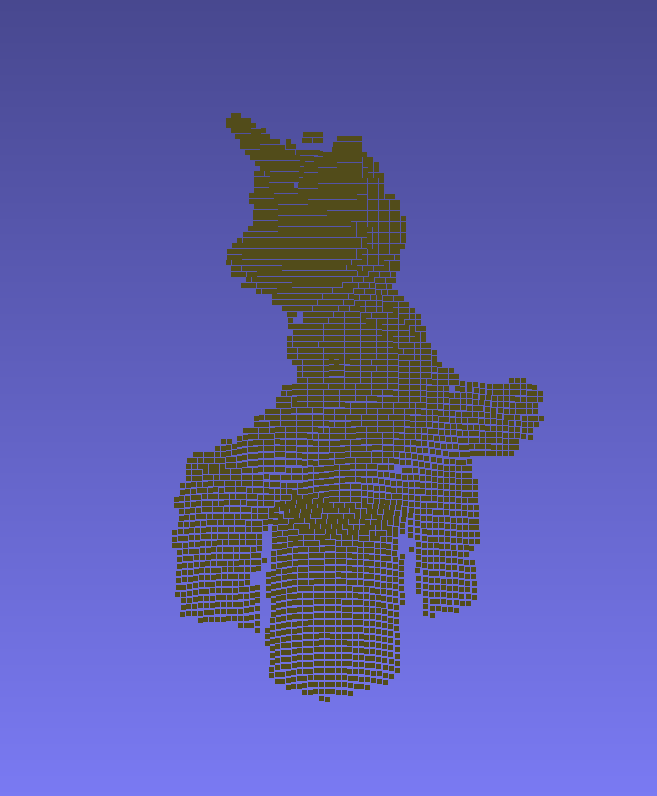
\includegraphics[height=4cm]{archivos/ejemplo-acumulacion-transformacion-captura-1.png}
        % Captura 1, 2 y 3 pero la 1 superpuesta por encima
        \caption{Captura 1.}
        \label{fig:ejemplo-acumulacion-transformacion-captura-1}
    \end{subfigure}
    \begin{subfigure}[t]{0.2\textheight}
    	\centering
        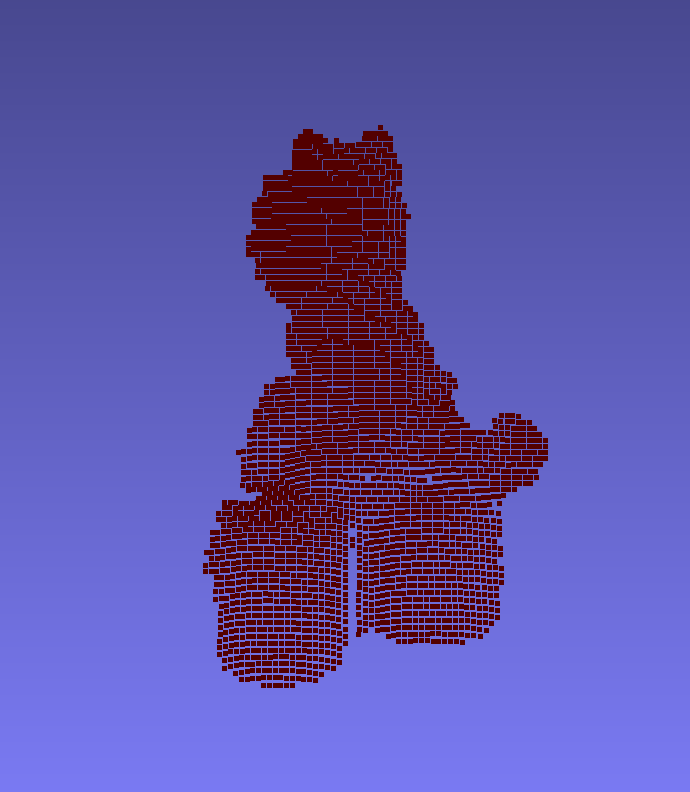
\includegraphics[height=4cm]{archivos/ejemplo-acumulacion-transformacion-captura-2.png}
        % Captura 1, 2 y 3 pero la 2 superpuesta por encima
        \caption{Captura 2.}
        \label{fig:ejemplo-acumulacion-transformacion-captura-2}
    \end{subfigure}
    \begin{subfigure}[t]{0.2\textheight}
    	\centering
        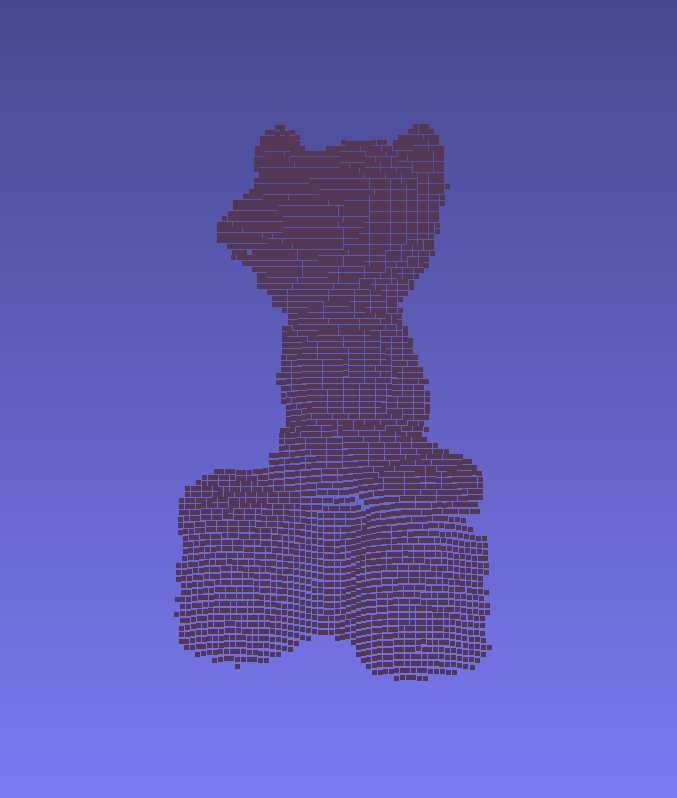
\includegraphics[height=4cm]{archivos/ejemplo-acumulacion-transformacion-captura-3.png}
        % Captura 1, 2 y 3 pero la 3 superpuesta por encima
        \caption{Captura 3.}
        \label{fig:ejemplo-acumulacion-transformacion-captura-3}
    \end{subfigure}
    \begin{subfigure}[t]{0.2\textheight}
    	\centering
        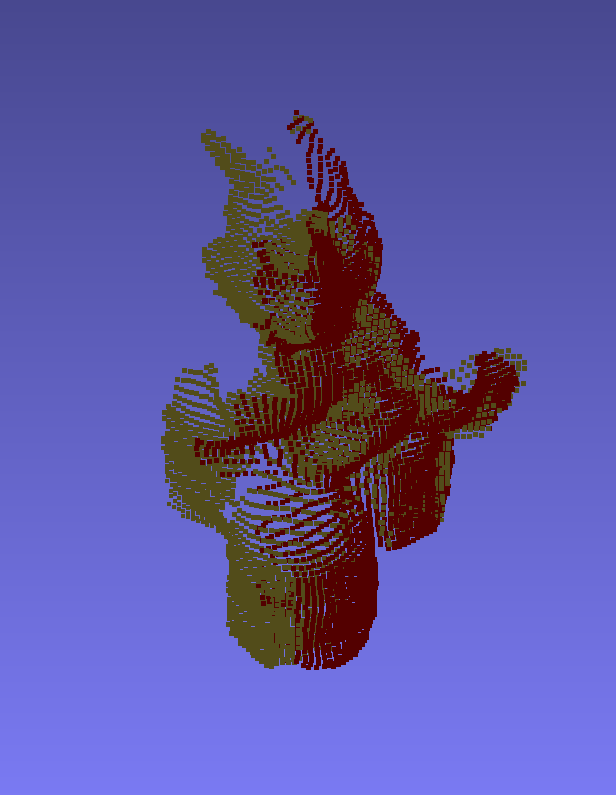
\includegraphics[height=4cm]{archivos/ejemplo-acumulacion-transformacion-captura-2-alineada.png}
        % Captura 1 y 2 alineadas y la 3, pero la 1 y 2 superpuestas por encima
        \caption{Captura 2 (escena) alineada con la captura 1 (modelo).}
        \label{fig:ejemplo-acumulacion-transformacion-captura-2-alineada}
    \end{subfigure}
    \begin{subfigure}[t]{0.2\textheight}
    	\centering
        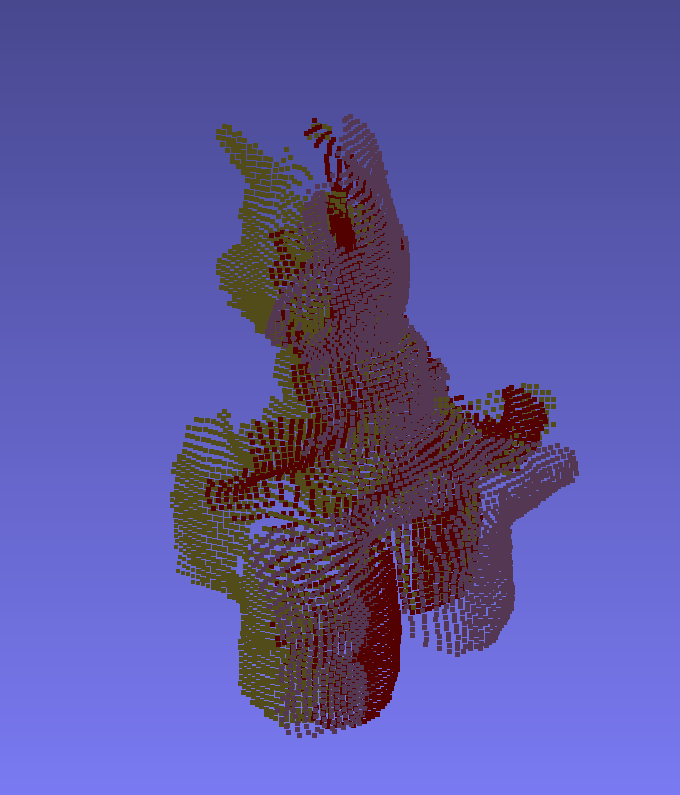
\includegraphics[height=4cm]{archivos/ejemplo-acumulacion-transformacion-captura-3-transformacion-inicial.png}
        % Captura 1 y 2 alineadas y la 3, 3 superpuesta por encima
        \caption{Captura 3 con transformación inicial.}
        \label{fig:ejemplo-acumulacion-transformacion-captura-3-transformacion-inicial}
    \end{subfigure}
    \begin{subfigure}[t]{0.2\textheight}
    	\centering
        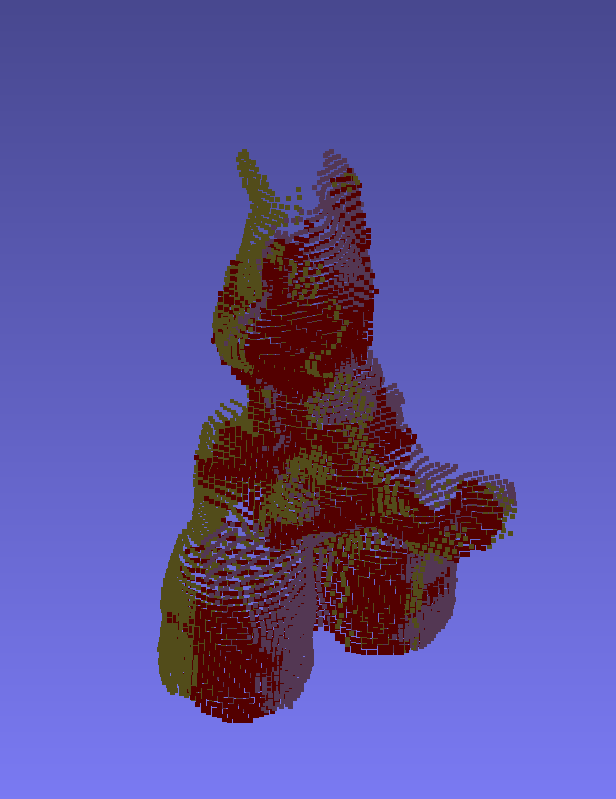
\includegraphics[height=4cm]{archivos/ejemplo-acumulacion-transformacion-captura-3-alineada.png}
        % Captura 1, 2 y 3 alineadas
        \caption{Captura 3 (escena) alineada con 1 y 2 (modelo).}
        \label{fig:ejemplo-acumulacion-transformacion-captura-3-alineada}
    \end{subfigure}
    \caption{Ejemplo de matriz de transformación inicial.}
    \label{fig:ejemplo-acumulacion-transformacion}
\end{figure}

\section{Filtros para el pre-procesamiento y post-procesamiento de los datos}

Tras la fase de adquisición, donde obtenemos una nube de puntos que identificamos como modelo y el resto de nube de puntos que identificamos como escenas, es buena idea hacer uso de filtros sobre las nubes de puntos en una fase de pre-procesamiento antes de ser enviadas al método de registro donde serán finalmente procesadas.
Esto puede ayudar al método de registro para que funcione mejor encontrando las correspondencias entre las nubes de puntos.

Además, tras ser procesadas por el método de registro, también se puede volver a aplicar otros filtros en una fase de post-procesamiento. Este filtro de post-procesamiento puede ayudar a obtener un resultado de mayor calidad para la fase final de análisis.

En la Figura \ref{fig:diagrama-filtros-pre-post-procesamiento} podemos ver un esquema que muestra en qué momento se aplicarán los filtros de pre-procesamiento y post-procesamiento.

\begin{figure}[h]
    \centering
    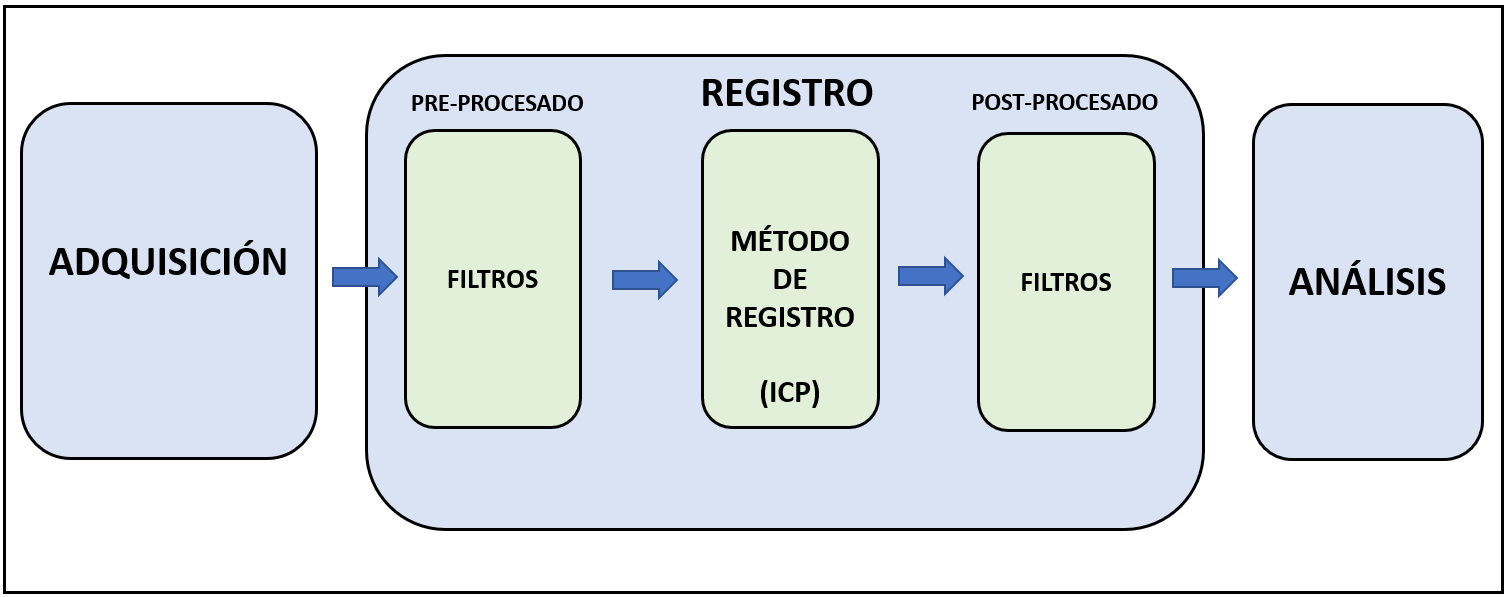
\includegraphics[height=6cm]{archivos/diagrama-filtros-pre-post-procesamiento.png}
    \caption{Filtros de pre-procesamiento y post-procesamiento en un esquema general de un sistema 3D.}
    \label{fig:diagrama-filtros-pre-post-procesamiento}
\end{figure}

A continuación, se detallarán una serie de filtros que se aplicarán en fase de pre-procesado que harán que el método de registro funcione mejor.

\begin{description}

    \item[Filtro de diezmado (Decimation Filter):]
    
    el filtro de diezmado ayuda a eliminar el exceso de ancho de banda y reduce la frecuencia de muestreo de la señal a una frecuencia de muestreo más baja que difiere de la frecuencia original en un valor entero.
    También ayuda a reducir los recursos computacionales necesarios para procesar y almacenar la señal \citep{engineerAmbitiosly}.

    La razón para aplicar este filtro normalmente consiste en reducir la frecuencia de muestreo en la salida de un sistema para que un sistema que opera a una frecuencia de muestreo más baja pueda ingresar la señal.
    Pero una motivación mucho mayor para diezmar, y motivo por el cual es interesante para este proyecto, es reducir el costo de procesamiento al tratar con los datos tras ser aplicado el filtro. Gracias a este filtro obtenemos una nube de puntos con menor cantidad de puntos, lo cual permitirá al método de registro trabajar más rápido.

    Este filtro es muy parecido al downsampling, sin perder demasiada calidad en la nube de puntos. El uso de este filtro está recomendado en la documentación de Intel, y proporcionan un método en la librería de RealSense para aplicarlo a la hora de tomar la captura.
    
    % \item[Reducción de muestreo (Downsampling):]
    
    % el filtro consiste en reducir la cantidad total de puntos en la muestra, obteniendo solo un conjunto de datos de nube de puntos, utilizando un enfoque de cuadrícula voxelizada.

    % La implementación de este filtro por \gls{pcl} consiste en crear una cuadrícula de vóxeles\footnote{Un vóxel es la unidad cúbica que compone un objeto tridimensional. Constituye la unidad mínima procesable de una matriz tridimensional y es, por tanto, el equivalente del píxel en un objeto 2D.} 3D sobre los datos de la nube de puntos de entrada.
    % Luego, en cada vóxel, se aproximarán todos los puntos presentes con su centroide.
    % Este enfoque es un poco más lento que aproximarlos con el centro del vóxel, pero representa la superficie subyacente con mayor precisión.

    % Por tanto, con la aplicación de este filtro obtendremos una nube de puntos más reducida pero con la suficiente calidad para que el método de registro funcione adecuadamente.    

    \item[PassThrough Filter:]
    
    este filtro consiste en definir unos valores para cada dimensión donde la nube de puntos será recortada.
    Es decir, se especifica un rango para las dimensiones $\mathbf{X}$, $\mathbf{Y}$, $\mathbf{Z}$, y todo lo que esté fuera de dicho rango será recortado de la nube de puntos.

    Con este filtro conseguimos por una parte, reducir la cantidad de puntos finales, con lo que conseguimos una nube de puntos más liviana y, como se ha comentado en los filtros anteriores, esto hará que el método de registro funcione más rápido.
    Pero lo más importante es que podemos eliminar la parte de la nube de puntos que no nos interesa y que, además, podría entorpecer en el funcionamiento del método de registro.
    Por ejemplo, si lo que estamos capturando con el sensor es una persona dando vueltas en el mismo sitio, todos los objetos, paredes y entorno que le rodea no es información relevante para el registro.
    De hecho, puede provocar un peor funcionamiento si se dejara, pues son puntos fijos que no cambian entre captura y captura.

    \item[Statistical Outlier Removal Filter:]
    
    este filtro es muy interesante porque nos permite eliminar valores atípicos en la nube de puntos, que probablemente serán mediciones ruidosas que ha capturado el sensor.
    Los errores de medición en la fase de adquisición conducen a valores atípicos dispersos que corrompen los resultados del registro.

    La eliminación estadística de valores atípicos funciona realizando un análisis estadístico de la vecindad de cada punto y recortando aquellos que no cumplen con un determinado criterio.
    La eliminación de valores atípicos dispersos se basa en el cálculo de la distribución de puntos a distancias vecinas en el conjunto de datos de entrada.
    Para cada punto, se calcula la distancia media desde él a todos sus vecinos.
    Todos los puntos cuyas distancias medias están fuera de un intervalo definido por la media y la desviación estándar de las distancias globales pueden considerarse valores atípicos y recortarse del conjunto de datos.

    Por tanto el uso de este filtro nos permite obtener una nube de puntos más limpia eliminando los puntos lejanos, puntos atípicos y que no corresponden con el objeto o cuerpo capturado.

    \item[Filtro de mediana (Median Filter):]
    
    El filtro de la mediana es uno de los filtros de procesamiento de imágenes más simples y más extendidos, se sabe que funciona bien con ruido de disparo o ruido de impulso.\footnote{El ruido de disparo o de impulso son píxeles individuales que tienen valores extremos.}
    Es simple de implementar y eficiente, ya que requiere una sola pasada sobre la imagen. Consiste en una ventana móvil de tamaño fijo que reemplaza el píxel del centro por la mediana dentro de la ventana.

\end{description}

Los filtros de eliminación estadística de valores atípico (Statistical Outlier Removal) y de mediana también son filtros muy interesantes para aplicar en la fase de post-procesado, ya que además de permitir un mejor funcionamiento durante el método de registro, mejora la calidad de la nube de puntos resultante.

\section{Aceleración por GPU, CUDA}

Los métodos de registro \gls{2d} y \gls{3d} suelen proporcionar buenos resultados, sin embargo presentan restricciones temporales debido a su naturaleza secuencial y a la gran cantidad de cálculos que deben realizar.
Es por ello que se buscan métodos para acelerar dichos algoritmos que minimicen todo lo posible las restricciones temporales.
La forma tradicional de aceleración aplicada a estos métodos es la computación paralela.

El paradigma \gls{gpgpu} \citep{Luebke2006} es un concepto dentro de la informática que trata de estudiar y aprovechar las capacidades de cómputo de una \gls{gpu}.
Inicialmente los dispositivos \gls{gpu} se utilizaban únicamente para el procesamiento de los gráficos de un ordenador cuyos datos a tratar estaban enfocados a ser convertidos a formato gráfico.
En la actualidad combinan su gran potencia de cálculo para albergar cálculos paralelos de propósito general en los que se trabaja con grandes cantidades de datos que no tienen por qué ser convertidos a formato gráfico.

Existen dos tecnologías principales para la programación en dispositivos \gls{gpu}: \glsentryfull{cuda} y \gls{opencl}.
En un principio la programación para aprovechar las características de este tipo de dispositivos debía hacerse mediante código ensamblador.
Sin embargo, hoy día existen alternativas con lenguajes de alto nivel que facilitan el desarrollo de las aplicaciones.
\gls{cuda} \citep{Luebke2008} es una plataforma de computación en paralelo que incluye un compilador y un conjunto de herramientas de desarrollo creadas por Nvidia que permite utilizar una variación del lenguaje de programación C (CUDA C) para codificar algoritmos en \gls{gpu}s de Nvidia.
\gls{opencl} \citep{Stone2010} por su parte consta de una interfaz de programación de aplicaciones y de un lenguaje de programación que permiten crear aplicaciones con paralelismo a nivel de datos y de tareas que pueden ejecutarse en \gls{gpu}.
Se trata de una alternativa a \gls{cuda} de código libre y abierta.

Los dispositivos \gls{gpu}s consiguen mejor rendimiento que las \gls{cpu}s procesando datos en coma flotante debido a su arquitectura.
Como podemos ver en la Figura \ref{fig:comparacion-cpu-gpu} \citep{Stopper2017}, un dispositivo \gls{gpu} está diseñado para el cálculo intensivo altamente paralelo, por lo que tiene más transistores destinados al procesamiento de datos que al flujo de control o a la caché de datos.
Las \gls{gpu}s son dispositivos especialmente adecuados para resolver problemas que puedan expresarse como cálculos con datos realizados
simultáneamente, ejecutando el mismo programa sobre muchos datos en paralelo.
Los cálculos que se realizan conllevan una alta intensidad aritmética, es decir, un elevado ratio de operaciones aritméticas por operación de memoria, lo que hace innecesaria la utilización de grandes cantidades de caché de datos.

\begin{figure}[h]
    \centering
    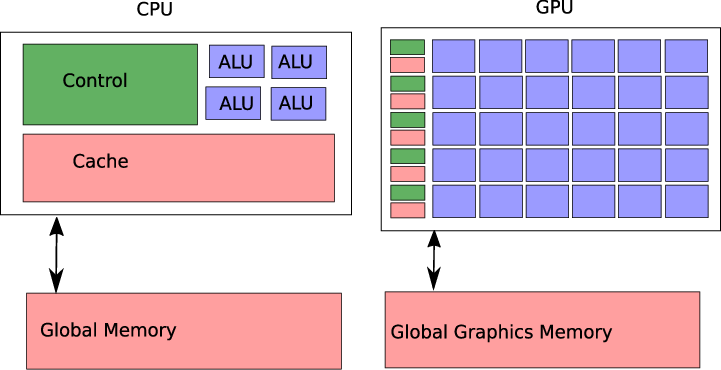
\includegraphics[width=0.7\linewidth]{archivos/comparativa-cpu-gpu.png}
    \caption{Comparación de arquitecturas CPU y GPU. Figura extraída de \cite{Stopper2017}.}
    \label{fig:comparacion-cpu-gpu}
\end{figure}

\gls{cuda} es una arquitectura con modelo \gls{simt}, es decir, una instrucción, múltiples hilos.
Estos hilos se ejecutan simultáneamente, trabajando sobre grandes cantidades de datos en paralelo.
En la Figura \ref{fig:arquitectura-gpu-cuda} \citep{peter2009nvidia} podemos ver la estructura de los dispositivos \gls{gpu} compatibles con la arquitectura \gls{cuda}, los cuales están formados por un conjunto de multiprocesadores.
Estos multiprocesadores reciben el nombre de \gls{sm} y permiten trabajar con múltiples hilos en paralelo.
Sin embargo, el número de multiprocesadores varía dependiendo de la arquitectura de la \gls{gpu}. Cada \gls{sm} se compone de una serie de \gls{sp} que comparten la lógica de control y la memoria caché.
Cada uno de estos \gls{sp} puede lanzar una gran cantidad de hilos en paralelo.

\begin{figure}[h]
    \centering
    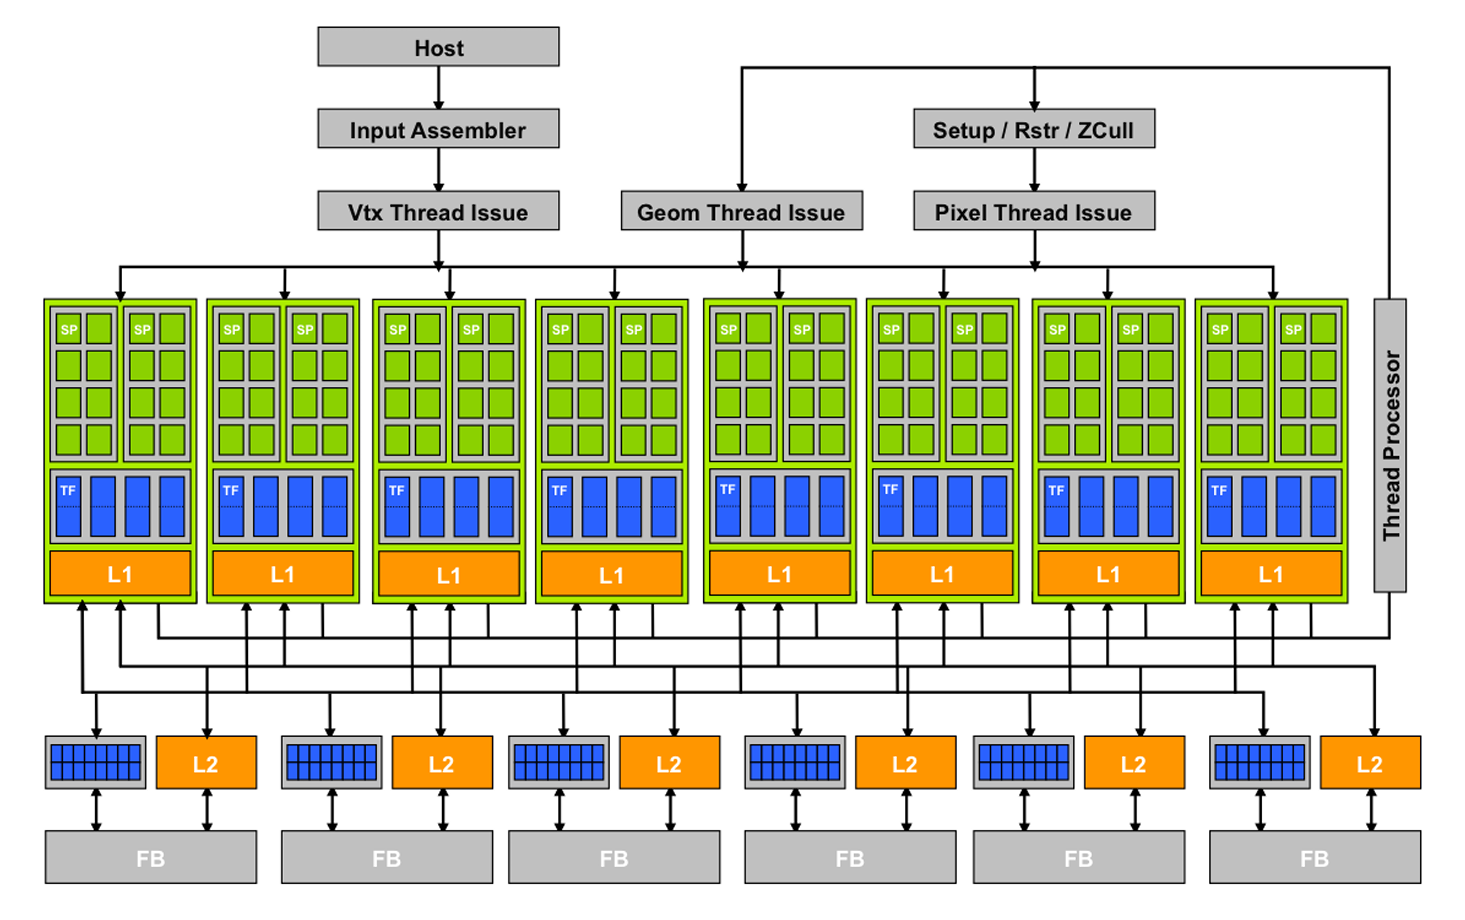
\includegraphics[width=\linewidth]{archivos/diagrama-arquitectura-cuda.png}
    \caption{Arquitectura GPU con tecnología CUDA. Figura extraída de \cite{peter2009nvidia}.}
    \label{fig:arquitectura-gpu-cuda}
\end{figure}

Una vez definida la importancia de los dispositivos \gls{gpu} para la resolución de problemas de cálculo intensivo a los que se aplican computación paralela, para utilizar estos dispositivos con el objetivo de acelerar un determinado algoritmo será necesario realizar un rediseño del algoritmo que se adapte a la arquitectura de la \gls{gpu}.
Para paralelizar un algoritmo de forma eficiente será necesario identificar claramente unidades de trabajo independientes capaces de trabajar con subconjuntos de datos.
Este es un aspecto crítico a la hora de rediseñar un algoritmo para que funcione concurrentemente.

El algoritmo \gls{icp} requiere mucho tiempo de proceso en la \gls{cpu} debido a la gran cantidad de operaciones que deben realizar en cada una de sus etapas, concretamente la encargada de calcular los emparejamientos entre las nubes de puntos escena y modelo.
En esta etapa es donde se encuentra el principal cuello de botella del algoritmo \gls{icp}, ya que el algoritmo debe encontrar para cada punto de la escena el punto del modelo más cercano.
Esta etapa del algoritmo realizada en la \gls{cpu} de forma secuencial emplea una gran cantidad de tiempo.
Muchas de estas operaciones se pueden realizar en paralelo ya que son independientes y trabajan sobre el mismo conjunto de datos, lo cual hace que el algoritmo cumpla con los requisitos básicos para poder ser implementado de forma paralela, orientado a su ejecución en una \gls{gpu}, de esta manera se puede reducir notablemente el tiempo de procesamiento que emplea el algoritmo.

Existen varias implementaciones desarrolladas en \gls{gpu} del algoritmo \gls{icp} \citep{Langis} \citep{barsukov2013development}.
Incluso Nvidia ha creado oficialmente un repositorio con implementaciones sobre la librería \gls{pcl}, incluyendo una implementación sobre el algoritmo \gls{icp} \citep{LeiFan}.
